\documentclass[]{article}
\usepackage{lmodern}
\usepackage{amssymb,amsmath}
\usepackage{ifxetex,ifluatex}
\usepackage{fixltx2e} % provides \textsubscript
\ifnum 0\ifxetex 1\fi\ifluatex 1\fi=0 % if pdftex
  \usepackage[T1]{fontenc}
  \usepackage[utf8]{inputenc}
\else % if luatex or xelatex
  \ifxetex
    \usepackage{mathspec}
  \else
    \usepackage{fontspec}
  \fi
  \defaultfontfeatures{Ligatures=TeX,Scale=MatchLowercase}
\fi
% use upquote if available, for straight quotes in verbatim environments
\IfFileExists{upquote.sty}{\usepackage{upquote}}{}
% use microtype if available
\IfFileExists{microtype.sty}{%
\usepackage{microtype}
\UseMicrotypeSet[protrusion]{basicmath} % disable protrusion for tt fonts
}{}
\usepackage[margin=1in]{geometry}
\usepackage{hyperref}
\hypersetup{unicode=true,
            pdftitle={UML Notes},
            pdfborder={0 0 0},
            breaklinks=true}
\urlstyle{same}  % don't use monospace font for urls
\usepackage{longtable,booktabs}
\usepackage{graphicx,grffile}
\makeatletter
\def\maxwidth{\ifdim\Gin@nat@width>\linewidth\linewidth\else\Gin@nat@width\fi}
\def\maxheight{\ifdim\Gin@nat@height>\textheight\textheight\else\Gin@nat@height\fi}
\makeatother
% Scale images if necessary, so that they will not overflow the page
% margins by default, and it is still possible to overwrite the defaults
% using explicit options in \includegraphics[width, height, ...]{}
\setkeys{Gin}{width=\maxwidth,height=\maxheight,keepaspectratio}
\IfFileExists{parskip.sty}{%
\usepackage{parskip}
}{% else
\setlength{\parindent}{0pt}
\setlength{\parskip}{6pt plus 2pt minus 1pt}
}
\setlength{\emergencystretch}{3em}  % prevent overfull lines
\providecommand{\tightlist}{%
  \setlength{\itemsep}{0pt}\setlength{\parskip}{0pt}}
\setcounter{secnumdepth}{0}
% Redefines (sub)paragraphs to behave more like sections
\ifx\paragraph\undefined\else
\let\oldparagraph\paragraph
\renewcommand{\paragraph}[1]{\oldparagraph{#1}\mbox{}}
\fi
\ifx\subparagraph\undefined\else
\let\oldsubparagraph\subparagraph
\renewcommand{\subparagraph}[1]{\oldsubparagraph{#1}\mbox{}}
\fi

%%% Use protect on footnotes to avoid problems with footnotes in titles
\let\rmarkdownfootnote\footnote%
\def\footnote{\protect\rmarkdownfootnote}

%%% Change title format to be more compact
\usepackage{titling}

% Create subtitle command for use in maketitle
\providecommand{\subtitle}[1]{
  \posttitle{
    \begin{center}\large#1\end{center}
    }
}

\setlength{\droptitle}{-2em}

  \title{UML Notes}
    \pretitle{\vspace{\droptitle}\centering\huge}
  \posttitle{\par}
    \author{}
    \preauthor{}\postauthor{}
    \date{}
    \predate{}\postdate{}
  
\usepackage{graphicx} \usepackage{subcapitaion}

\begin{document}
\maketitle

\hypertarget{paradigmi-oop}{%
\section{Paradigmi OOP}\label{paradigmi-oop}}

\begin{enumerate}
\def\labelenumi{\arabic{enumi}.}
\item
  \textbf{Abstraction:} usare le classi per astrarre la natura delle
  caratteristiche di un oggetto, eche é un'istanza della propria classe
  di appartenenza.
\item
  \textbf{Encapsulation:} Nascondere i dettagli del funzionamento di un
  oggetto; gli oggetti hanno accesso solo ai dati che hanno bisogno.
\item
  \textbf{Inheritance:} classi possono specializzare altre classi
  ereditando da esse e implementando solo la porzione di comportamento
  che differisce.
\item
  \textbf{Polynorohism:} invocare comportamento diverso in reazione allo
  stesso messaggio, a seconda di quell'oggetto che lo riceve.
\end{enumerate}

\hypertarget{diagrammie-e-viste}{%
\section{Diagrammie e viste}\label{diagrammie-e-viste}}

Un diagramma è la rappresentazione grafica di un modello e fornisce una
vista di un sistema (o una sua parte) per metterne in risalto le sue
proprietà.

Viste:

\begin{enumerate}
\def\labelenumi{\arabic{enumi}.}
\item
  \textbf{Logical:} mette in risalto la scomposizione logica del sistema
  tramite classi, oggetti e loro relazioni.
\item
  \textbf{Development:} mostra l'organizzazione del sistema in blocchi
  strutturali (packages, sottosistemi, librerie, \ldots).
\item
  \textbf{Process:} mostra i processi (o thread) del sistema in
  funzione, e le loro interazioni.
\item
  \textbf{Physical:} mostra come il sistema viene installato se eseguito
  fisicamente.
\item
  \textbf{Use case:} spiega il funzionamento desiderato del sistema.
\end{enumerate}

UML fornisce i diagrammi divisi in due categorie:

\begin{itemize}
\item
  \textbf{Structure diagrams:} come è fatto il sistema; fornisce le
  vieste \emph{Logical}, \emph{Development} e \emph{Physical}.
\item
  \textbf{Behaviot diagrams:} come funziona il sistema; fornisce le
  viste \emph{Process} e \emph{Use case}.
\end{itemize}

\begin{longtable}[]{@{}ll@{}}
\toprule
Structure & Behavior\tabularnewline
\midrule
\endhead
Class diagram & Use Case diagram\tabularnewline
Object diagram & Activity diagram\tabularnewline
Package diagram & State Machine diagram\tabularnewline
Composite Structure diagram & Sequence diagram\tabularnewline
Component diagram & Communication diagram\tabularnewline
Deployment diagram & Interaction Overview diagram\tabularnewline
& Timing diagram\tabularnewline
\bottomrule
\end{longtable}

\hypertarget{primitive-di-uml}{%
\section{Primitive di UML}\label{primitive-di-uml}}

Contiene tre tipi di elementi le cui sottoclassi possono apparire nei
diagrammi:

\begin{itemize}
\tightlist
\item
  \textbf{Classifier:} é un insieme di \textbf{things}.
\item
  \textbf{Event;} é un insieme di possibili avvenimenti
  (\emph{occurrences}).
\item
  \textbf{Behaviour:} è un insieme di esecuzioni (\emph{executions}).
\end{itemize}

\hypertarget{entita-strutturali}{%
\section{Entità strutturali}\label{entita-strutturali}}

\begin{figure}
    \centering
    \begin{subfigure}[b]{0.3\textwidth}
        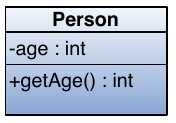
\includegraphics[width=\textwidth]{img/Classe.png}
        \caption{Esempio di classe.}
        %\label{fig:gull}
    \end{subfigure}
    \begin{subfigure}[b]{0.3\textwidth}
        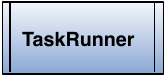
\includegraphics[width=\textwidth]{img/Active.png}
        \caption{Esempio di Active Class.}
        %\label{fig:tiger}
    \end{subfigure}
    \begin{subfigure}[b]{0.3\textwidth}
        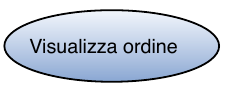
\includegraphics[width=\textwidth]{img/Usecase.png}
        \caption{Esempio di Use Case.}
        %\label{fig:mouse}
    \end{subfigure}
    \caption{Entità strutturali.}
    %\label{fig:animals}
\end{figure}


\end{document}
